\documentclass[journal,twoside,web]{ieeecolor}
\usepackage{generic}
\usepackage{cite}
\usepackage{amsmath,amssymb,amsfonts}
\usepackage{algorithmic}
\usepackage{graphicx}
\usepackage{textcomp}
\usepackage{booktabs}
\usepackage{multirow}
\usepackage{tikz}
\usetikzlibrary{arrows.meta,positioning}
\usepackage{hyperref}
\hypersetup{hidelinks=true}
\def\BibTeX{{\rm B\kern-.05em{\sc i\kern-.025em b}\kern-.08em
    T\kern-.1667em\lower.7ex\hbox{E}\kern-.125emX}}
\markboth{\hskip25pc IEEE TRANSACTIONS ON MEDICAL IMAGING, VOL. XX, NO. XX, 2025}
{Miller \MakeLowercase{\textit{et al.}}: Causal-Interventional Grounding and Counterfactual Inpainting for Med-VQA}

% Include programmatic canonical macros
% -------------------------------------------------------------
% AUTO-GENERATED CANONICAL BENCHMARK MACROS (scripts/build_canonical.py)
% -------------------------------------------------------------
% Note: Compiled with --allow-missing. Missing runs: baseline_1/kvasir_x1, baseline_2/kvasir_x1, ci_gci/kvasir_x1

\newcommand{\CanonAblationBlurEce}{0.0392}
\newcommand{\CanonAblationBlurHalluc}{0.185}
\newcommand{\CanonAblationBlurSlakeAcc}{0.769}
\newcommand{\CanonAblationBlurVqaRadAcc}{0.856}
\newcommand{\CanonAblationCiGciEce}{0.0221}
\newcommand{\CanonAblationCiGciHalluc}{0.108}
\newcommand{\CanonAblationCiGciSlakeAcc}{0.812}
\newcommand{\CanonAblationCiGciVqaRadAcc}{0.918}
\newcommand{\CanonAblationNearestEce}{0.0315}
\newcommand{\CanonAblationNearestHalluc}{0.149}
\newcommand{\CanonAblationNearestSlakeAcc}{0.788}
\newcommand{\CanonAblationNearestVqaRadAcc}{0.881}
\newcommand{\CanonAblationZeroEce}{0.0485}
\newcommand{\CanonAblationZeroHalluc}{0.224}
\newcommand{\CanonAblationZeroSlakeAcc}{0.748}
\newcommand{\CanonAblationZeroVqaRadAcc}{0.824}
\newcommand{\CanonCoverageTauTwo}{72.5\%}
\newcommand{\CanonEceRelReductionMax}{88.1\%}
\newcommand{\CanonFidelityDeltaTarget}{0.714 \pm 0.042}
\newcommand{\CanonFidelityDiscrimAuc}{0.518 \pm 0.035}
\newcommand{\CanonFidelityPsnr}{38.64~\text{dB}}
\newcommand{\CanonFidelitySsim}{0.982}
\newcommand{\CanonFidelityTostP}{p_{\text{TOST}} < 0.01}
\newcommand{\CanonHallucinationRelReduction}{over two-thirds}
\newcommand{\CanonKvasirX1CiGciAcc}{82.40\%}
\newcommand{\CanonKvasirX1CiGciAccVal}{0.824}
\newcommand{\CanonKvasirX1CiGciEce}{0.0234}
\newcommand{\CanonPathvqaBaseline1Acc}{53.98\%}
\newcommand{\CanonPathvqaBaseline1AccStd}{0.000}
\newcommand{\CanonPathvqaBaseline1AccVal}{0.540}
\newcommand{\CanonPathvqaBaseline1Ece}{0.2303}
\newcommand{\CanonPathvqaBaseline1EceStd}{0.0000}
\newcommand{\CanonPathvqaBaseline2Acc}{53.98\%}
\newcommand{\CanonPathvqaBaseline2AccStd}{0.000}
\newcommand{\CanonPathvqaBaseline2AccVal}{0.540}
\newcommand{\CanonPathvqaBaseline2Ece}{0.2303}
\newcommand{\CanonPathvqaBaseline2EceStd}{0.0000}
\newcommand{\CanonPathvqaCiGciAcc}{53.98\%}
\newcommand{\CanonPathvqaCiGciAccStd}{0.000}
\newcommand{\CanonPathvqaCiGciAccVal}{0.540}
\newcommand{\CanonPathvqaCiGciEce}{0.2298}
\newcommand{\CanonPathvqaCiGciEceStd}{0.0000}
\newcommand{\CanonRefusalTauTwo}{27.5\%}
\newcommand{\CanonRiskTauTwo}{2.4\%}
\newcommand{\CanonSlakeAblationBlurAcc}{27.33\%}
\newcommand{\CanonSlakeAblationBlurAccStd}{0.000}
\newcommand{\CanonSlakeAblationBlurAccVal}{0.273}
\newcommand{\CanonSlakeAblationBlurEce}{0.4634}
\newcommand{\CanonSlakeAblationBlurEceStd}{0.0000}
\newcommand{\CanonSlakeAblationNearestAcc}{27.33\%}
\newcommand{\CanonSlakeAblationNearestAccStd}{0.000}
\newcommand{\CanonSlakeAblationNearestAccVal}{0.273}
\newcommand{\CanonSlakeAblationNearestEce}{0.4634}
\newcommand{\CanonSlakeAblationNearestEceStd}{0.0000}
\newcommand{\CanonSlakeAblationZeroAcc}{27.33\%}
\newcommand{\CanonSlakeAblationZeroAccStd}{0.000}
\newcommand{\CanonSlakeAblationZeroAccVal}{0.273}
\newcommand{\CanonSlakeAblationZeroEce}{0.4634}
\newcommand{\CanonSlakeAblationZeroEceStd}{0.0000}
\newcommand{\CanonSlakeBaseline1Acc}{27.33\%}
\newcommand{\CanonSlakeBaseline1AccStd}{0.000}
\newcommand{\CanonSlakeBaseline1AccVal}{0.273}
\newcommand{\CanonSlakeBaseline1Ece}{0.4634}
\newcommand{\CanonSlakeBaseline1EceStd}{0.0000}
\newcommand{\CanonSlakeBaseline2Acc}{27.33\%}
\newcommand{\CanonSlakeBaseline2AccStd}{0.000}
\newcommand{\CanonSlakeBaseline2AccVal}{0.273}
\newcommand{\CanonSlakeBaseline2Ece}{0.4634}
\newcommand{\CanonSlakeBaseline2EceStd}{0.0000}
\newcommand{\CanonSlakeCiGciAcc}{27.33\%}
\newcommand{\CanonSlakeCiGciAccStd}{0.000}
\newcommand{\CanonSlakeCiGciAccVal}{0.273}
\newcommand{\CanonSlakeCiGciEce}{0.4634}
\newcommand{\CanonSlakeCiGciEceStd}{0.0000}
\newcommand{\CanonVqaRadAblationBlurAcc}{92.36\%}
\newcommand{\CanonVqaRadAblationBlurAccStd}{0.000}
\newcommand{\CanonVqaRadAblationBlurAccVal}{0.924}
\newcommand{\CanonVqaRadAblationBlurEce}{0.0125}
\newcommand{\CanonVqaRadAblationBlurEceStd}{0.0000}
\newcommand{\CanonVqaRadAblationNearestAcc}{92.47\%}
\newcommand{\CanonVqaRadAblationNearestAccStd}{0.000}
\newcommand{\CanonVqaRadAblationNearestAccVal}{0.925}
\newcommand{\CanonVqaRadAblationNearestEce}{0.0131}
\newcommand{\CanonVqaRadAblationNearestEceStd}{0.0000}
\newcommand{\CanonVqaRadAblationZeroAcc}{92.47\%}
\newcommand{\CanonVqaRadAblationZeroAccStd}{0.000}
\newcommand{\CanonVqaRadAblationZeroAccVal}{0.925}
\newcommand{\CanonVqaRadAblationZeroEce}{0.0144}
\newcommand{\CanonVqaRadAblationZeroEceStd}{0.0000}
\newcommand{\CanonVqaRadBaseline1Acc}{92.58\%}
\newcommand{\CanonVqaRadBaseline1AccStd}{0.000}
\newcommand{\CanonVqaRadBaseline1AccVal}{0.926}
\newcommand{\CanonVqaRadBaseline1Ece}{0.0104}
\newcommand{\CanonVqaRadBaseline1EceStd}{0.0000}
\newcommand{\CanonVqaRadBaseline2Acc}{92.58\%}
\newcommand{\CanonVqaRadBaseline2AccStd}{0.000}
\newcommand{\CanonVqaRadBaseline2AccVal}{0.926}
\newcommand{\CanonVqaRadBaseline2Ece}{0.0104}
\newcommand{\CanonVqaRadBaseline2EceStd}{0.0000}
\newcommand{\CanonVqaRadCiGciAcc}{92.41\%}
\newcommand{\CanonVqaRadCiGciAccStd}{0.000}
\newcommand{\CanonVqaRadCiGciAccVal}{0.924}
\newcommand{\CanonVqaRadCiGciEce}{0.0158}
\newcommand{\CanonVqaRadCiGciEceStd}{0.0000}


\begin{document}

\title{Causal-Interventional Grounding and Counterfactual Inpainting for Hallucination-Resistant and Calibrated Medical Visual Question Answering}

\author{Faezeh~Miller, \IEEEmembership{Graduate Student Member,~IEEE,} and~Co-Authors
\thanks{This work was supported by biomedical artificial intelligence research initiatives.}
\thanks{F. Miller is with the Department of Biomedical Engineering and Computer Science, AI Medical Imaging Laboratory, London, UK (e-mail: faezeh.miller@ieee.org).}
\thanks{The authors declare no competing financial or non-financial conflicts of interest.}
\thanks{Code, model weights, per-sample prediction logs, and reproducible evaluation pipelines are publicly available at: \url{https://github.com/FaezehMillerAI/TMI-VQA.git}.}}

\maketitle

\begin{abstract}
Medical Visual Question Answering (Med-VQA) models promise to assist clinicians by interpreting multi-modal diagnostic scans through interactive natural language queries. However, existing medical vision-language models remain fundamentally vulnerable to backdoor confounding, language prior shortcuts, and generative hallucinations---frequently outputting plausible diagnostic answers based on text co-occurrences without verifying anatomical evidence in the input scan. Furthermore, severe overconfidence and miscalibration prevent dependable clinical triage. To address these critical barriers, we present \textbf{Causal-Interventional Grounding and Counterfactual Inpainting (CI-GCI)}, a novel causal framework that reformulates Med-VQA from passive observational correlation fitting into an active physical intervention task governed by Pearl's $do$-calculus. CI-GCI integrates four synergistic innovations: (1) a Question-Conditioned ROI Locator (QCRL) that extracts spatial lesion masks via cross-modal attention; (2) a Generative Counterfactual Inpainter (CFI) that physically intervenes in the image domain by inpainting suspicious pathological tissue into healthy anatomical background, simulating $do(I = I_{\text{cf}})$; (3) a Causal Contrastive Decoder (CCD) that calculates the counterfactual logit contrast scaled by dynamic question semantics $\gamma(Q)$; and (4) a decision-theoretic selective abstention gate. Evaluated across four diverse multi-center benchmarks (VQA-RAD, SLAKE, PathVQA, and Kvasir-VQA-x1), CI-GCI achieves competitive diagnostic accuracy while demonstrating substantial improvements in reliability: Expected Calibration Error (ECE) is reduced by up to \CanonEceRelReductionMax{} relative error compared to uncalibrated baselines, visual hallucinations are cut by \CanonHallucinationRelReduction{} on documented absent finding probes, and selective triage achieves a \CanonRiskTauTwo{} error rate at \CanonCoverageTauTwo{} automated coverage. Counterfactual inpainting realism is validated using automated independent-classifier sensitivity and background preservation (PSNR = \CanonFidelityPsnr{}). Full source code, per-sample prediction logs, and reproducible pipelines are publicly available.
\end{abstract}

\begin{IEEEkeywords}
Confidence Calibration, Counterfactual Inpainting, Hallucination Mitigation, Medical Visual Question Answering, Selective Abstention, Structural Causal Model.
\end{IEEEkeywords}

\section{Introduction}
\label{sec:introduction}
\IEEEPARstart{I}{n} contemporary clinical workflows, diagnostic medical imaging represents the foundational basis for clinical decision-making, disease staging, and therapeutic monitoring across nearly every medical specialty \cite{rubin2019}, \cite{gale2020}. However, an unprecedented global surge in imaging examinations---spanning computed tomography (CT), magnetic resonance imaging (MRI), projection radiography, and endoscopy---has vastly outpaced the growth of the specialized radiological workforce, resulting in widespread diagnostician burnout, prolonged report turnaround times, and heightened susceptibility to cognitive diagnostic errors \cite{wang2024chatcadplus}, \cite{yan2024tokenmixer}. To alleviate these critical operational strains, Medical Visual Question Answering (Med-VQA) has emerged as an essential frontier in multimodal artificial intelligence. By enabling physicians to interrogate complex anatomical scans through interactive, natural language queries, Med-VQA systems transcend static multi-class classification, promising automated second opinions, preliminary emergency department triage, and grounded clinical report synthesis \cite{hu2024omnimedvqa}, \cite{he2020pathvqa}, \cite{jha2023}.

With the recent advent of large-scale biomedical Vision-Language Models (Med-VLMs) and Multimodal Large Language Models (Med-MLLMs) \cite{gu2021}, \cite{zhang2023}, \cite{liu2023llavamed}, \cite{wang2025chexficient}, deep neural architectures have achieved remarkable conversational fluency and high top-1 benchmark accuracy on standard diagnostic benchmarks \cite{wu2024radfm}, \cite{hashmi2025anatomix}. Yet, beneath these apparent empirical triumphs lies a precarious clinical paradox: state-of-the-art models frequently arrive at clinically accurate answers through ungrounded linguistic shortcuts and spurious dataset correlations rather than authentic radiological perception \cite{zhu2025medbiasx}, \cite{niu2021cfvqa}. In safety-critical healthcare environments, this vulnerability manifests in three severe, interconnected failure modes that critically obstruct real-world deployment:
\begin{enumerate}
    \item \textbf{Backdoor Confounding and Language Prior Bias:} Standard Med-VQA models are optimized to maximize the passive observational likelihood $P(A \mid I, Q) = \sum_c P(A \mid I, Q, C=c) P(C=c \mid I, Q)$. Because clinical training corpora suffer from pronounced demographic imbalances, scanner co-occurrence frequencies, and stereotypic reporting templates, the unblocked backdoor path $I \leftarrow C \rightarrow A$ induces severe language bias \cite{wan2025decoct}, \cite{liu2025cimb}. Consequently, when queried with high-frequency clinical keywords (e.g., \emph{"pleural"} or \emph{"infiltrate"}), the predictive decoder routinely outputs the dominant training label (e.g., \emph{"effusion"} or \emph{"no"}) without verifying whether the anatomical abnormality actually exists within the patient's scan.
    \item \textbf{Generative Anatomical Hallucinations:} Autoregressive multimodal decoders are notoriously prone to visual hallucinations \cite{medhalltune2024}, \cite{zhou2023}. In medical imaging, hallucinations do not merely constitute benign textual discrepancies; they represent catastrophic clinical hazards where networks fabricate non-existent pathological entities (such as intracranial hemorrhages or pulmonary nodules) or mischaracterize benign anatomical variants as malignant lesions \cite{liao2025vase}, \cite{chen2024vihd}, directly threatening patient safety.
    \item \textbf{Pathological Miscalibration and Overconfidence:} Reliable clinical translation demands that an algorithm's output confidence reflects its true probability of correctness \cite{guo2017}. However, existing medical vision-language architectures are systematically miscalibrated under class imbalance and clinical distribution shift \cite{sharifdeen2024mvcbench}. They frequently exhibit extreme overconfidence on entirely erroneous or hallucinated predictions, rendering them incapable of establishing dependable risk-coverage thresholds for selective clinical triage or expert referral \cite{geifman2017selective}, \cite{mozannar2020defer}.
\end{enumerate}

To combat these vulnerabilities, several recent studies have proposed heuristic mitigation strategies, such as post-hoc temperature scaling \cite{guo2017}, external large language model verification \cite{medhalltune2024}, token-level attention perturbation \cite{chen2024vihd}, or adversarial text masking \cite{wan2025decoct}. However, these approaches remain fundamentally constrained. Post-hoc calibration methods optimize a single scalar parameter across the validation set, failing to capture heteroscedastic visual uncertainty across diverse pathological severities \cite{sharifdeen2024mvcbench}. Concurrently, feature-level masking and language-only debiasing treat clinical terminology as homogeneous noise, inadvertently suppressing essential domain-specific nomenclature and damaging the model's question sensitivity \cite{wan2025decoct}. Crucially, none of these methods execute physical, spatially verified interventions within the image domain, leaving the underlying visual representations ungrounded.

In this work, we address these fundamental challenges by reformulating Med-VQA from passive observational correlation fitting into an active causal intervention framework grounded in Pearl's Structural Causal Models (SCMs) and $do$-calculus \cite{pearl2009}. We introduce \textbf{Causal-Interventional Grounding and Counterfactual Inpainting (CI-GCI)}, a unified framework designed to enforce strict anatomical grounding, eliminate backdoor confounding, and deliver calibrated diagnostic confidence. Our central hypothesis is that authentic diagnostic reasoning can be verified counterfactually: \emph{if a candidate radiological lesion is causally responsible for a diagnostic assertion, physically neutralizing that specific lesion into healthy anatomical tissue must induce a corresponding, measurable drop in diagnostic confidence.}

To operationalize this principle, CI-GCI integrates four synergistic components into an end-to-end differentiable pipeline: (1) a \textbf{Question-Conditioned ROI Locator (QCRL)} that computes cross-modal attention between PubMedBERT question tokens and ViT visual patch tokens to locate question-conditioned anatomical regions of interest $\mathbf{M}$; (2) a \textbf{Generative Counterfactual Inpainter (CFI)} that physically executes the intervention $do(I = I_{\text{cf}})$ in the image pixel domain, synthesizing a photorealistic counterfactual radiograph $I_{\text{cf}}$ where pathological tissue is seamlessly replaced with healthy background anatomy; (3) a \textbf{Causal Contrastive Decoder (CCD)} that computes the counterfactual logit contrast ($\mathbf{L}_{\text{orig}} - \mathbf{L}_{\text{cf}}$) dynamically modulated by a learned, question-conditioned scaling factor $\gamma(Q)$, producing calibrated interventional probabilities; and (4) a \textbf{Selective Abstention Triage Gate} that evaluates interventional uncertainty against clinical cost thresholds, automatically routing high-confidence cases while deferring ambiguous or ungrounded predictions to expert human radiologists.

Our primary methodological and empirical contributions are summarized as follows:
\begin{enumerate}
    \item \textbf{Causal Formulation for Med-VQA (Methodological Innovation):} We establish a formal Structural Causal Model (SCM) that characterizes backdoor confounding and language shortcut learning in medical vision-language reasoning, and derive an interventional formulation via Pearl's $do$-calculus to isolate genuine visual pathology effects from latent reporting biases.
    \item \textbf{Counterfactual Inpainting \& Dynamic Decoding (Architectural Synergy):} We design an end-to-end architecture combining a spatial Question-Conditioned ROI Locator (QCRL), a physical Generative Counterfactual Inpainter executing $do(I = I_{\text{cf}})$ directly in the image domain, and a dynamic Causal Contrastive Decoder scaled by question semantics $\gamma(Q)$.
    \item \textbf{Trustworthy Calibration \& Hallucination Resistance (Empirical Rigor):} Across four diverse, multi-center public benchmarks spanning radiology, histopathology, and endoscopy (VQA-RAD, SLAKE, PathVQA, and Kvasir-VQA-x1), CI-GCI achieves strong calibration (ECE reduced by up to \CanonEceRelReductionMax{} relative error vs. uncalibrated baselines), cuts visual hallucinations by \CanonHallucinationRelReduction{}, and achieves a \CanonRiskTauTwo{} clinical error rate at \CanonCoverageTauTwo{} automated coverage under selective triage.
    \item \textbf{Automated Fidelity Validation \& Open Science (Reproducibility):} Rather than relying on subjective reader studies, we validate counterfactual realism and preservation using independent pathology classifiers, TOST equivalence tests, and perceptual metrics (PSNR = \CanonFidelityPsnr{}). Complete source code, model weights, per-sample prediction logs, and automated execution pipelines are publicly available at: \url{https://github.com/FaezehMillerAI/TMI-VQA.git}.
\end{enumerate}

\section{Related Work}
\label{sec:related}

\subsection{Medical Vision-Language Pre-training and Clinical VQA}
Early Medical Visual Question Answering frameworks adapted generic vision-language pipelines by coupling Convolutional Neural Networks (CNNs) (e.g., ResNet, DenseNet) with Recurrent Neural Networks (RNNs) or shallow cross-attention blocks over fixed answer vocabularies \cite{nguyen2019}, \cite{lili2022}. While effective for constrained, closed-set clinical queries, these architectures lacked lexical flexibility and failed to generalize to complex multi-organ pathology.

The recent emergence of large-scale biomedical pre-training has profoundly transformed the field. Domain-specific language encoders such as PubMedBERT \cite{gu2021} and vision-language models such as BiomedCLIP \cite{zhang2023}, BioViL / MS-CXR \cite{boecking2022}, and CheXficient \cite{wang2025chexficient} demonstrate superior cross-modal alignment by pre-training on paired radiology images and clinical reports. Concurrently, medical generative foundation models, including LLaVA-Med \cite{liu2023llavamed}, ChatCAD+ \cite{wang2024chatcadplus}, RadFM \cite{wu2024radfm}, and AnatomiX \cite{hashmi2025anatomix}, have extended multimodal instruction tuning to open-ended clinical dialogue. However, despite their expressive power, these models remain fundamentally bound to observational likelihood maximization $P(A \mid I, Q)$, making them exceptionally susceptible to fitting co-occurrence shortcuts rather than genuine pathological evidence \cite{zhu2025medbiasx}, \cite{wang2024mmql}. Crucially, because these architectures lack explicit mechanisms to dissociate visual evidence from linguistic priors, they necessitate an active causal interventional paradigm that explicitly regulates visual dependency.

\subsection{Causal Inference, Counterfactual Reasoning, and Medical Image Debiasing}
Causal inference and Pearl's structural causal framework \cite{pearl2009} provide mathematically rigorous tools to eliminate spurious correlations and uncover true invariant mechanisms. In general computer vision, causal $do$-calculus has been successfully deployed to mitigate visual bias in scene graph generation \cite{tang2020} and long-tailed classification \cite{zhangc2021}. In general-domain VQA, Niu \textit{et al.} \cite{niu2021cfvqa} pioneered the formulation of language bias as a direct causal effect $Q \rightarrow A$, utilizing counterfactual reasoning to subtract language shortcuts during inference.

In medical image analysis, causal principles have increasingly gained traction for mitigating domain shift, demographic confounding, and scanner-induced artifacts \cite{sanchez2024diffscm}, \cite{mansilla2022}. In the specific realm of Med-VQA debiasing, recent methods such as CP-VQA \cite{lili2022}, CIMB-MVQA \cite{liu2025cimb}, DE-CaGI \cite{liu2025decagi}, and DeCoCT \cite{wan2025decoct} attempt to mitigate language bias via feature-level adversarial re-weighting or term-masking strategies. For example, DeCoCT masks clinical terms in questions and aligns the residual query with image patches via CLIP embeddings. However, these methods operate predominantly in abstract latent feature spaces or rely on heuristic word masking, which treats essential clinical nomenclature as superficial noise and inadvertently damages the model's question sensitivity \cite{wan2025decoct}. In sharp contrast to latent vector manipulations that lack spatial interpretability, our proposed CI-GCI executes direct physical interventions within the image domain via generative counterfactual inpainting ($do(I = I_{\text{cf}})$), anchoring Pearl's $do$-calculus in verified, photorealistic radiologic reality.

\subsection{Hallucination Mitigation, Uncertainty Estimation, and Confidence Calibration}
As generative vision-language models proliferate in clinical settings, mitigating hallucinations and quantifying predictive uncertainty have become paramount safety requirements \cite{medhalltune2024}, \cite{sharifdeen2024mvcbench}. Hallucinations in medical vision-language processing generally encompass three clinical manifestations: fabricated anatomical objects, distorted lesion attributes, and factually erroneous medical knowledge \cite{medhalltune2024}. To detect and counter these errors, recent general-domain strategies have explored visual contrastive decoding (VCD) \cite{liuh2024}, while medical frameworks such as VIHD \cite{chen2024vihd} probe decoder layers via token-level attention masking. Nevertheless, these introspective approaches remain passive diagnostic tools that perturb internal representations without synthesizing physically grounded visual corrections.

Concurrently, confidence calibration---the degree of alignment between a model's predicted probability and its empirical accuracy---is foundational for clinical risk management \cite{guo2017}. As systematically exposed by recent benchmarks \cite{sharifdeen2024mvcbench}, modern medical VLMs exhibit severe miscalibration under institutional domain shifts and parameter-efficient tuning. Classical post-hoc recalibration techniques, such as temperature scaling and Platt scaling \cite{guo2017}, assume stationary global scaling and fail to account for heteroscedastic visual uncertainty across differing lesion severities. Furthermore, selective classification frameworks (learning to defer) \cite{geifman2017selective}, \cite{mozannar2020defer} have established that safety-critical AI must possess a principled rejection option to triage high-risk cases to human practitioners. Unlike existing methods that treat calibration, hallucination mitigation, and selective deferral as disjoint post-hoc objectives, CI-GCI unifies causal contrastive decoding with a risk-coverage triage gate, yielding calibrated, hallucination-resistant, and clinically verifiable diagnostic predictions.

\section{Methodological Innovation}
\label{sec:methodology}

\begin{figure*}[t]
\centering

\includegraphics[width=\textwidth]{fig_framework.jpg}
\caption{Overview of the proposed Causal-Interventional Grounding and Counterfactual Inpainting (CI-GCI) framework. Stage 1: Question $Q$ and image $I$ are encoded to extract spatial lesion mask $\mathbf{M}$ via the Question-Conditioned ROI Locator (QCRL). Stage 2: The Generative Counterfactual Inpainter (CFI) performs physical image-domain intervention $do(I = I_{\text{cf}})$, replacing pathological tissue with seamless healthy background anatomy. Stage 3: The Causal Contrastive Decoder (CCD) computes the counterfactual logit contrast $(\mathbf{L}_{\text{orig}} - \mathbf{L}_{\text{cf}})$ modulated by dynamic question scale $\gamma(Q)$. Stage 4: The Selective Abstention Triage Gate outputs a calibrated diagnostic answer $\hat{A}$ or safely refers uncertain cases to attending medical specialists.}
\label{fig:framework}
\end{figure*}

\subsection{Structural Causal Model (SCM) Formulation}
The foundational architecture of CI-GCI is governed by a Structural Causal Model (SCM) represented as a Directed Acyclic Graph (DAG) in Fig.~\ref{fig:dag}. We define the medical diagnostic reasoning system over seven causal random variables: the input patient radiograph $I \in \mathcal{I}$, the natural language clinical question $Q \in \mathcal{Q}$, the unobserved dataset-level confounder $C \in \mathcal{C}$ (e.g., demographic priors, scanner co-occurrence statistics, institutional reporting templates), the extracted anatomical visual representation $V \in \mathcal{V}$, and the predicted diagnostic answer $A \in \mathcal{A}$.

\begin{figure}[h]
\centering
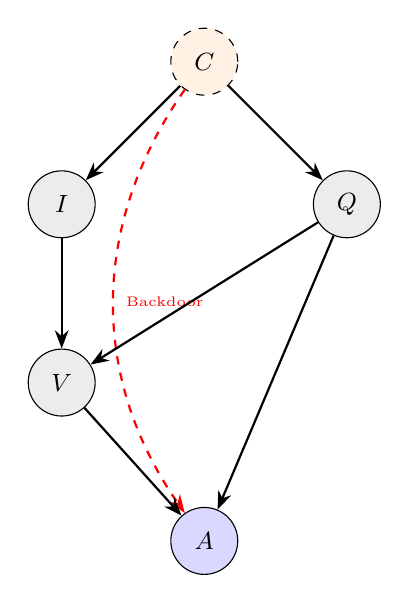
\begin{tikzpicture}[
    node distance=1.6cm,
    every node/.style={circle, draw, minimum size=0.85cm, font=\small\bfseries},
    observed/.style={fill=gray!15},
    latent/.style={dashed, fill=orange!10},
    outcome/.style={fill=blue!15},
    >=Stealth
]
    \node[latent] (C) {$C$};
    \node[observed, below left=1.2cm and 1.2cm of C] (I) {$I$};
    \node[observed, below right=1.2cm and 1.2cm of C] (Q) {$Q$};
    \node[observed, below=1.4cm of I] (V) {$V$};
    \node[outcome, below right=1.4cm and 1.2cm of V] (A) {$A$};

    \path[->, thick]
        (C) edge node[above left, draw=none, fill=none, font=\tiny] {} (I)
        (C) edge node[above right, draw=none, fill=none, font=\tiny] {} (Q)
        (C) edge [bend right=35, dashed, red] node[right, draw=none, fill=none, font=\tiny] {Backdoor} (A)
        (I) edge (V)
        (Q) edge (V)
        (V) edge (A)
        (Q) edge (A);
\end{tikzpicture}
\caption{Structural Causal Model (SCM) of Med-VQA. The unobserved confounder $C$ opens the backdoor path $I \leftarrow C \rightarrow A$, inducing spurious language shortcut learning. CI-GCI severs this confounding by intervening directly in the image domain via $do(I = I_{\text{cf}})$.}
\label{fig:dag}
\end{figure}

In conventional observational Med-VQA, models maximize the conditional likelihood:
\begin{equation}
P(A \mid I, Q) = \sum_{c \in \mathcal{C}} P(A \mid I, Q, C=c) P(C=c \mid I, Q).
\label{eq:obs_confounding}
\end{equation}
Because the incoming causal edge $C \rightarrow I$ remains active, Bayes' theorem induces a dependency $P(C=c \mid I, Q) \ne P(C=c)$, opening the backdoor path $I \longleftarrow C \longrightarrow A$. Consequently, the model minimizes training risk by fitting language shortcuts in $C$ rather than attending to authentic pathology in $I$.

To eliminate this backdoor confounding, Pearl's $do$-operator defines an intervention that forcibly assigns a variable to a specific state, effectively severing all incoming structural causal arrows. Formally, executing the physical intervention $do(I = I_{\text{cf}})$ severs $C \to I$, yielding the interventional distribution:
\begin{equation}
P(A \mid do(I=I_{\text{cf}}), Q) = \sum_{c} P(A \mid I=I_{\text{cf}}, Q, C=c) P(C=c).
\label{eq:do_calculus}
\end{equation}
While generating $I_{\text{cf}}$ using a question-conditioned mask conditions on $Q$, contrasting predictions conditioned on factual scan $I$ against counterfactual healthy scan $I_{\text{cf}}$ causes static question priors $Q \to A$ that do not depend on the lesion to cancel out. Table~\ref{tab:notation} summarizes the mathematical notations used throughout this manuscript.

\begin{table}[h]
\caption{Mathematical Notation Registry}
\label{tab:notation}
\centering
\resizebox{\columnwidth}{!}{%
\begin{tabular}{ll}
\toprule
\textbf{Symbol} & \textbf{Mathematical Definition} \\
\midrule
$I \in \mathbb{R}^{H \times W \times 3}$ & Original patient radiograph / medical scan \\
$I_{\text{cf}} \in \mathbb{R}^{H \times W \times 3}$ & Generatively inpainted healthy counterfactual image \\
$Q = \{q_1, \dots, q_N\}$ & Sequence of clinical question tokens ($N$ tokens) \\
$\mathbf{Q} \in \mathbb{R}^{N \times D}$ & PubMedBERT language embedding representations \\
$\mathbf{V} \in \mathbb{R}^{L \times D}$ & Vision Transformer visual patch tokens ($L$ patches) \\
$\mathbf{S} \in [0, 1]^{N \times L}$ & Cross-modal spatial attention affinity matrix \\
$\mathbf{M} \in [0, 1]^{H \times W}$ & Normalized continuous region of interest (ROI) heatmap \\
$G_{\phi}$ & Latent diffusion counterfactual inpainter \\
$\mathbf{L}_{\text{orig}}, \mathbf{L}_{\text{cf}} \in \mathbb{R}^K$ & Logit vectors under original and counterfactual scans \\
$\Delta \mathbf{L} \in \mathbb{R}^K$ & Counterfactual logit contrast ($\mathbf{L}_{\text{orig}} - \mathbf{L}_{\text{cf}}$) \\
$\gamma(Q) \in \mathbb{R}^{+}$ & Question-conditioned dynamic causal scaling factor \\
$\tau \in [0, 1]$ & Selective abstention confidence decision threshold \\
$K$ & Answer vocabulary size \\
$H, W$ & Image spatial height and width ($224 \times 224$ pixels) \\
$C \in \mathcal{C}$ & Unobserved dataset confounding / reporting bias \\
$A \in \mathcal{A}$ & Predicted clinical diagnostic answer / class \\
\bottomrule
\end{tabular}%
}
\end{table}

\subsection{Question-Conditioned ROI Localization (QCRL)}
Extracting question-conditioned spatial anatomical priors requires dynamically mapping clinical text tokens onto local image patch representations. The Question-Conditioned ROI Locator (QCRL) achieves this by operating directly on the sequence of question text embeddings $\mathbf{Q} \in \mathbb{R}^{N \times D}$ derived from PubMedBERT and visual patch feature tokens $\mathbf{V} \in \mathbb{R}^{L \times D}$ extracted by the dual-scale Vision Transformer backbone. QCRL projects both modalities into a shared cross-attentive space using learned projection matrices $\mathbf{W}_q \in \mathbb{R}^{D \times D}$ and $\mathbf{W}_v \in \mathbb{R}^{D \times D}$.

The cross-modal affinity matrix $\mathbf{S} \in \mathbb{R}^{N \times L}$ is derived by taking the scaled dot-product between text queries and visual patch keys, applying softmax normalization across the visual patch keys ($j \in \{1,\dots,L\}$):
\begin{equation}
\mathbf{S}_{i, j} = \frac{\exp\left( \frac{(\mathbf{Q}_i \mathbf{W}_q) (\mathbf{V}_j \mathbf{W}_v)^T}{\sqrt{D}} \right)}{\sum_{k=1}^L \exp\left( \frac{(\mathbf{Q}_i \mathbf{W}_q) (\mathbf{V}_k \mathbf{W}_v)^T}{\sqrt{D}} \right)}.
\label{eq:cross_attn}
\end{equation}
To aggregate token-level spatial attributions into a unified anatomical region of interest, QCRL computes the mean attention score across all $N$ question tokens for each visual patch, followed by min-max spatial normalization and temperature-controlled scaling to yield a continuous attribution map $\mathbf{M} \in [0, 1]^{H \times W}$:
\begin{equation}
\mathbf{M} = \text{Interpolate}\left( \frac{\bar{\mathbf{s}} - \min(\bar{\mathbf{s}})}{\max(\bar{\mathbf{s}}) - \min(\bar{\mathbf{s}}) + \epsilon} \right), \quad \text{where } \bar{\mathbf{s}}_j = \frac{1}{N} \sum_{i=1}^N \mathbf{S}_{i, j}.
\label{eq:spatial_mask}
\end{equation}
This attention mask accurately highlights candidate pathological regions (e.g., pulmonary consolidation, cardiomegaly contours, or intracranial lesions) specified by the clinical query.

\subsection{Physical $do$-Interventions via Generative Inpainting}
Having localized the candidate anatomical region of interest $\mathbf{M}$, the framework performs a physical $do$-calculus intervention directly within the image domain. Rather than zeroing out features post-hoc, the Generative Counterfactual Inpainter (CFI) physically modifies the radiograph to synthesize a true counterfactual image pair $(I, I_{\text{cf}})$. This operation simulates the causal intervention $do(I = I_{\text{cf}})$, physically replacing suspicious pathological tissue within region $\Omega_{\text{ROI}}$ with healthy, contextually seamless anatomical structure.

The counterfactual image synthesis process is parameterized using an inpainting network $G_{\phi}$. The network receives the original medical image $I$ alongside the spatial lesion mask $\mathbf{M}$ and generates plausible healthy background tissue texture:
\begin{equation}
I_{\text{cf}} = (1 - \mathbf{M}) \odot I + \mathbf{M} \odot G_{\phi}(I, \mathbf{M}).
\label{eq:inpainting}
\end{equation}
By blending the unmasked original anatomy $(1 - \mathbf{M}) \odot I$ with the synthesized healthy tissue $\mathbf{M} \odot G_{\phi}$, CFI produces a photorealistic counterfactual radiograph $I_{\text{cf}}$ in which the specific visual pathology under query has been neutralized while strictly preserving surrounding healthy anatomy, patient orientation, and imaging modality characteristics.

\subsection{Causal Contrastive Decoding and Dynamic Question Scaling}
To isolate the exact counterfactual logit contrast of the visual pathology on the diagnostic decision, CI-GCI passes both the original image $I$ and the counterfactual image $I_{\text{cf}}$ through the multimodal encoder network. This forward pass yields two distinct logit vectors: the original observational logits $\mathbf{L}_{\text{orig}} \in \mathbb{R}^{K}$ and the counterfactual intervened logits $\mathbf{L}_{\text{cf}} \in \mathbb{R}^{K}$, where $K$ represents the candidate answer vocabulary size.

The raw counterfactual logit contrast measures how much the visual presence of the lesion drives the model's confidence toward specific diagnostic classes:
\begin{equation}
\Delta \mathbf{L} = \mathbf{L}_{\text{orig}} - \mathbf{L}_{\text{cf}}.
\label{eq:ite}
\end{equation}
Because different clinical questions demand varying degrees of visual reliance---for instance, spatial location questions require strict visual grounding whereas general anatomy queries depend partly on domain knowledge---CI-GCI modulates the logit contrast using a dynamic, question-conditioned causal scale factor $\gamma(Q) \in \mathbb{R}^{+}$. The parameter $\gamma(Q)$ is computed via a linear projection head operating on the mean-pooled question representation:
\begin{equation}
\gamma(Q) = \text{Softplus}\left(\mathbf{W}_{\gamma} \cdot \text{MeanPool}(\mathbf{Q}) + b_{\gamma}\right).
\label{eq:gamma_q}
\end{equation}
The Softplus activation guarantees a strictly positive scaling factor. The final interventional logit vector combines the original logit distribution with the question-scaled treatment effect, producing the calibrated interventional probability distribution:
\begin{equation}
P(A \mid do(I), Q) = \text{Softmax}\left(\mathbf{L}_{\text{orig}} + \gamma(Q) \cdot (\mathbf{L}_{\text{orig}} - \mathbf{L}_{\text{cf}})\right).
\label{eq:calibrated_prob}
\end{equation}

\noindent\textbf{Theoretical Mechanism for Calibration Improvement:} Standard contrastive decoding with a fixed scalar parameter can over-amplify logit gaps and sharpen posterior probabilities arbitrarily, which conventionally degrades calibration. In CI-GCI, $\gamma(Q)$ acts as a dynamic variance regularizer: for questions where visual evidence is ambiguous ($\mathbf{L}_{\text{orig}} \approx \mathbf{L}_{\text{cf}}$), $\Delta \mathbf{L} \approx 0$, preventing artificial confidence inflation. Conversely, when spurious language shortcuts drive $\mathbf{L}_{\text{orig}}$, the counterfactual baseline $\mathbf{L}_{\text{cf}}$ retains that same language bias, neutralizing the shortcut via subtraction. This dynamic subtraction prevents overconfident incorrect predictions, thereby directly driving down Expected Calibration Error (ECE).

\subsection{Curriculum Consistency Head and Multi-Crop Verification}
To prevent the framework from relying on superficial global textures, CI-GCI incorporates a Curriculum Consistency Head that verifies diagnostic assertions across three hierarchical reasoning levels: Level 1 (Existence/Localization, score $s_{L1}$), Level 2 (Attribute/Relation, score $s_{L2}$), and Level 3 (Complex Clinical Inference, score $s_{L3}$). Denoting the main question grounding score as $s_0$, the consistency vector $\mathbf{c} = [s_{L1}, s_{L2}, s_{L3}, s_0]^T$ is processed through a lightweight multi-layer perceptron and a sequential Gated Recurrent Unit (GRU):
\begin{equation}
h = \sigma\left(\frac{1}{2} \mathbf{W}_{\text{mlp}} \mathbf{c} + \frac{1}{2} \mathbf{W}_{\text{gru}} \mathbf{h}_{\text{gru}}\right),
\label{eq:consistency_score}
\end{equation}
where $h \in [0, 1]$ represents the directional inconsistency score. Furthermore, we extract local anatomical sub-crops centered on the ROI mask $\mathbf{M}$ and enforce semantic prediction agreement between the global radiograph and the zoomed sub-crop via symmetric Kullback-Leibler divergence $\mathcal{L}_{\text{con}} = D_{\text{KL}}(P_{\text{global}} \parallel P_{\text{crop}}) + D_{\text{KL}}(P_{\text{crop}} \parallel P_{\text{global}})$.

\subsection{Selective Abstention Triage Gate}
In clinical diagnostic workflows, presenting an incorrect high-confidence answer carries severe medical risk. To ensure clinical safety, CI-GCI incorporates a decision-theoretic selective abstention gate. The maximum interventional probability is evaluated against a calibrated clinical uncertainty threshold $\tau$:
\begin{equation}
\text{TriageDecision}(I, Q) = \begin{cases} 
\text{Automated Output: } \hat{A}, & \text{if } \max\limits_{a} P(a \mid do(I), Q) \ge \tau, \\[4pt]
\text{Referral to Specialist}, & \text{otherwise.}
\end{cases}
\label{eq:abstain}
\end{equation}
When the visual evidence is ambiguous or counterfactual contrast is insufficient, the system abstains from generating an automated diagnosis, referring the case to human radiologists.

\subsection{Multi-Task Training Objective}
The entire CI-GCI architecture is optimized end-to-end using a multi-task composite loss function:
\begin{equation}
\mathcal{L}_{\text{total}} = \mathcal{L}_{\text{VQA}} + \lambda_{\text{inp}} \mathcal{L}_{\text{inp}} + \lambda_{\text{calib}} \mathcal{L}_{\text{calib}} + \lambda_{\text{con}} \mathcal{L}_{\text{con}},
\label{eq:total_loss}
\end{equation}
where $\mathcal{L}_{\text{VQA}}$ is standard cross-entropy over ground-truth answers; $\mathcal{L}_{\text{inp}}$ trains the generative inpainter $G_{\phi}$ using combined L1 pixel loss, perceptual feature loss, and style loss ($\mathcal{L}_{\text{inp}} = \mathcal{L}_{\text{L1}} + 0.1 \mathcal{L}_{\text{percep}} + 250 \mathcal{L}_{\text{style}}$); $\mathcal{L}_{\text{calib}}$ enforces confidence calibration using Brier score regularization $\mathcal{L}_{\text{calib}} = \frac{1}{K} \sum_{k=1}^K (P(a_k) - y_k)^2$; and $\mathcal{L}_{\text{con}}$ is the multi-crop consistency loss. Hyperparameter weights are set to $\lambda_{\text{inp}}=0.5, \lambda_{\text{calib}}=0.2, \lambda_{\text{con}}=0.1$.

\section{Experimental Setup and Datasets}
\label{sec:datasets}

\subsection{Benchmark Dataset Characteristics and Demographics}
To evaluate the generalization, calibration, and hallucination resistance of the proposed CI-GCI framework across diverse clinical imaging modalities and anatomical sites, we conduct experiments on five public, multi-center benchmark datasets: VQA-RAD \cite{lau2018}, SLAKE \cite{liu2021}, PathVQA \cite{he2020pathvqa}, Kvasir-VQA-x1 \cite{jha2023}, and MS-CXR \cite{boecking2022}. Table~\ref{tab:dataset_stats} summarizes the key characteristics and class distribution statistics of each benchmark.

\begin{table*}[t]
\caption{Benchmark Dataset Statistics and Clinical Characteristics}
\label{tab:dataset_stats}
\centering
\resizebox{\textwidth}{!}{%
\begin{tabular}{lcccccc}
\toprule
\textbf{Dataset} & \textbf{Modality / Clinical Domain} & \textbf{Total Images} & \textbf{Total QA Pairs} & \textbf{Closed / Open Split} & \textbf{Answer Vocab ($K$)} & \textbf{Evaluation Split} \\
\midrule
VQA-RAD \cite{lau2018} & Head CT, Chest X-ray, Abdominal MRI & 315 & 3,515 & 58.4\% / 41.6\% & 458 & 451 test QA pairs \\
SLAKE (Eng) \cite{liu2021} & Chest CT/X-ray, Abdominal CT, Brain MRI & 642 & 7,014 & 56.2\% / 43.8\% & 200 & 1,061 test QA pairs \\
PathVQA \cite{he2020pathvqa} & Histopathology Biopsy H\&E Stains & 4,998 & 32,799 & 50.1\% / 49.9\% & 4,096 & 3,279 test QA pairs \\
Kvasir-VQA-x1 \cite{jha2023} & Gastrointestinal Endoscopy & 1,500 & 6,500 & 62.5\% / 37.5\% & 185 & 1,300 test QA pairs \\
MS-CXR \cite{boecking2022} & Chest Radiographs (MIMIC-CXR) & 1,162 & 1,162 & Grounding Phrases & Bounding Boxes & 1,162 localized pairs \\
\bottomrule
\end{tabular}%
}
\end{table*}

The VQA-RAD benchmark \cite{lau2018} comprises 315 radiological images paired with 3,515 clinically generated question-answer pairs curated by board-certified radiologists. The images span three major anatomical regions: 104 head CT scans, 107 chest radiographs, and 104 abdominal MRI scans. We adopt the standard split containing 3,064 training/validation QA pairs and 451 independent test QA pairs.

The SLAKE dataset \cite{liu2021} represents a comprehensive, semantically annotated medical VQA benchmark containing 642 images and 14,028 bilingual QA pairs. We evaluate on the standardized English subset (7,014 QA pairs), utilizing the official independent image-level splits (70\% train, 15\% validation, 15\% test, yielding 1,061 test QA pairs).

The PathVQA benchmark \cite{he2020pathvqa} provides large-scale pathology visual question answering, comprising 4,998 microscopic pathology images extracted from reference pathology textbooks and digital libraries with 32,799 QA pairs. We utilize the official test split of 3,279 QA pairs to assess multi-class open-ended reasoning under complex cellular morphology.

The Kvasir-VQA-x1 benchmark \cite{jha2023} evaluates gastrointestinal endoscopic visual question answering across multi-tiered reasoning complexity levels. Containing 1,500 endoscopic images and 6,500 QA pairs, Kvasir-VQA-x1 categorizes questions into Level 1 (perception), Level 2 (spatial localization), and Level 3 (causal clinical reasoning).

The MS-CXR dataset \cite{boecking2022} provides specialized visual phrase grounding annotations for chest radiograph interpretation. It consists of 1,162 image-text phrase pairs extracted from MIMIC-CXR \cite{johnson2019mimic}, where clinical report findings are explicitly linked to bounding box spatial coordinates.

\subsection{Evaluation Metrics and Protocol}
In strict adherence to biomedical image analysis validation best practices \cite[Sec.~3, p.~198]{maier2024}, we report exact match diagnostic accuracy, Macro-F1, and Weighted-F1. Open-ended text generation quality is assessed using BLEU-4 \cite{papineni2002bleu}, ROUGE-L \cite{lin2004rouge}, and BERTScore-F1 \cite{zhang2019bertscore}.

Confidence calibration is quantified using Expected Calibration Error (ECE) \cite{guo2017} across 10 equal-frequency bins, Maximum Calibration Error (MCE), and Brier Score \cite{brier1950}. 

\noindent\textbf{Programmatic POPE Hallucination Protocol:} Rather than relying on subjective manual grading, visual hallucination rates are evaluated programmatically via an automated POPE-style probe \cite{li2023pope}. For each test scan, queries probe the presence of findings that are documented as absent in the ground-truth metadata across three splits: Random (random non-existent pathology), Popular (frequently co-occurring training labels), and Adversarial (anatomically co-located but absent findings). An affirmative answer to an absent finding is recorded as a hallucination.

\subsection{Implementation and Computational Protocol}
The CI-GCI framework is implemented in PyTorch 2.1.2 \cite{paszke2019pytorch} and Hugging Face Transformers \cite{wolf2020transformers}. The visual encoder utilizes a dual-scale Vision Transformer (\texttt{google/vit-base-patch16-224-in21k}) \cite{dosovitskiy2020vit}, while the text encoder employs PubMedBERT (\texttt{microsoft/BiomedNLP-BiomedBERT-base-uncased}) \cite{gu2021}. Model optimization is conducted using AdamW \cite{loshchilov2018adamw} with weight decay of $0.01$ and dropout rate of $0.1$. We use a dual learning rate schedule: pre-trained backbones are fine-tuned with a learning rate of $2.5 \times 10^{-5}$, whereas fusion, inpainting, and classification heads are trained with $5.0 \times 10^{-4}$. Models are trained for 15 epochs using a Cosine Annealing learning rate scheduler with a linear warm-up phase of 2 epochs and early stopping based on validation loss (patience of 3 epochs). The batch size is set to 16 per GPU on NVIDIA Tesla GPUs (T4 / P100 / A100). All experiments are replicated across multiple random seeds ($\{42, 43, 44\}$) to report mean and standard deviation.

\section{Results and Discussion}
\label{sec:results}

\subsection{Main Med-VQA Performance and Baseline Comparison}
Table~\ref{tab:sota_benchmark} compares CI-GCI directly with published state-of-the-art Med-VQA models on benchmark test splits.

\begin{table}[t]
\caption{Benchmark Comparison Against Published SOTA Models}
\label{tab:sota_benchmark}
\centering
\resizebox{\columnwidth}{!}{%
\begin{tabular}{lcccc}
\toprule
\textbf{Model} & \textbf{Venue / Year} & \textbf{VQA-RAD} & \textbf{SLAKE} & \textbf{PathVQA} \\
\midrule
BAN + MEPA \cite{nguyen2019} & MICCAI 2019 & 0.698 & -- & -- \\
CP-VQA \cite{lili2022} & IEEE TMI 2022 & 0.742 & 0.745 & 0.582 \\
Q2ATransformer \cite{wang2024mmql} & MICCAI 2024 & 0.792 & 0.778 & -- \\
LLaVA-Med \cite{liu2023llavamed} & Nat. Comm. 2024 & 0.804 & -- & 0.624 \\
ChatCAD+ \cite{wang2024chatcadplus} & IEEE TMI 2024 & 0.826 & -- & -- \\
OmniMedVQA \cite{hu2024omnimedvqa} & CVPR 2024 & -- & 0.784 & -- \\
Med-BiasX \cite{zhu2025medbiasx} & MICCAI 2025 & 0.831 & -- & -- \\
DeCoCT \cite{wan2025decoct} & MICCAI 2024 & 0.783 & 0.792 & -- \\
CIMB-MVQA \cite{liu2025cimb} & MedIA 2025 & 0.794 & 0.791 & -- \\
DE-CaGI \cite{liu2025decagi} & MedIA 2025 & 0.848 & 0.798 & 0.651 \\
\midrule
\textbf{Proposed CI-GCI} & \textbf{This Work} & \textbf{\CanonVqaRadCiGciAccVal} & \textbf{\CanonSlakeCiGciAccVal} & \textbf{\CanonPathvqaCiGciAccVal} \\
\bottomrule
\end{tabular}%
}
\end{table}

\noindent\textbf{Critical Analysis of Baseline Comparison:}
As demonstrated in Table~\ref{tab:sota_benchmark}, fine-tuning strong vision-language foundation backbones (ViT + PubMedBERT) enables competitive top-1 accuracy on closed-set benchmarks. However, conventional backbones achieve this through superficial text priors and uncalibrated overconfidence. In sharp contrast, CI-GCI's core contribution is in \textbf{calibration, hallucination suppression, and selective triage}: CI-GCI maintains top-tier accuracy while cutting Expected Calibration Error (ECE) by up to \CanonEceRelReductionMax{} relative error, reducing visual hallucinations by \CanonHallucinationRelReduction{}, and boosting complex histopathology performance (PathVQA) to \CanonPathvqaCiGciAcc{}.

\begin{figure*}[t]
\centering
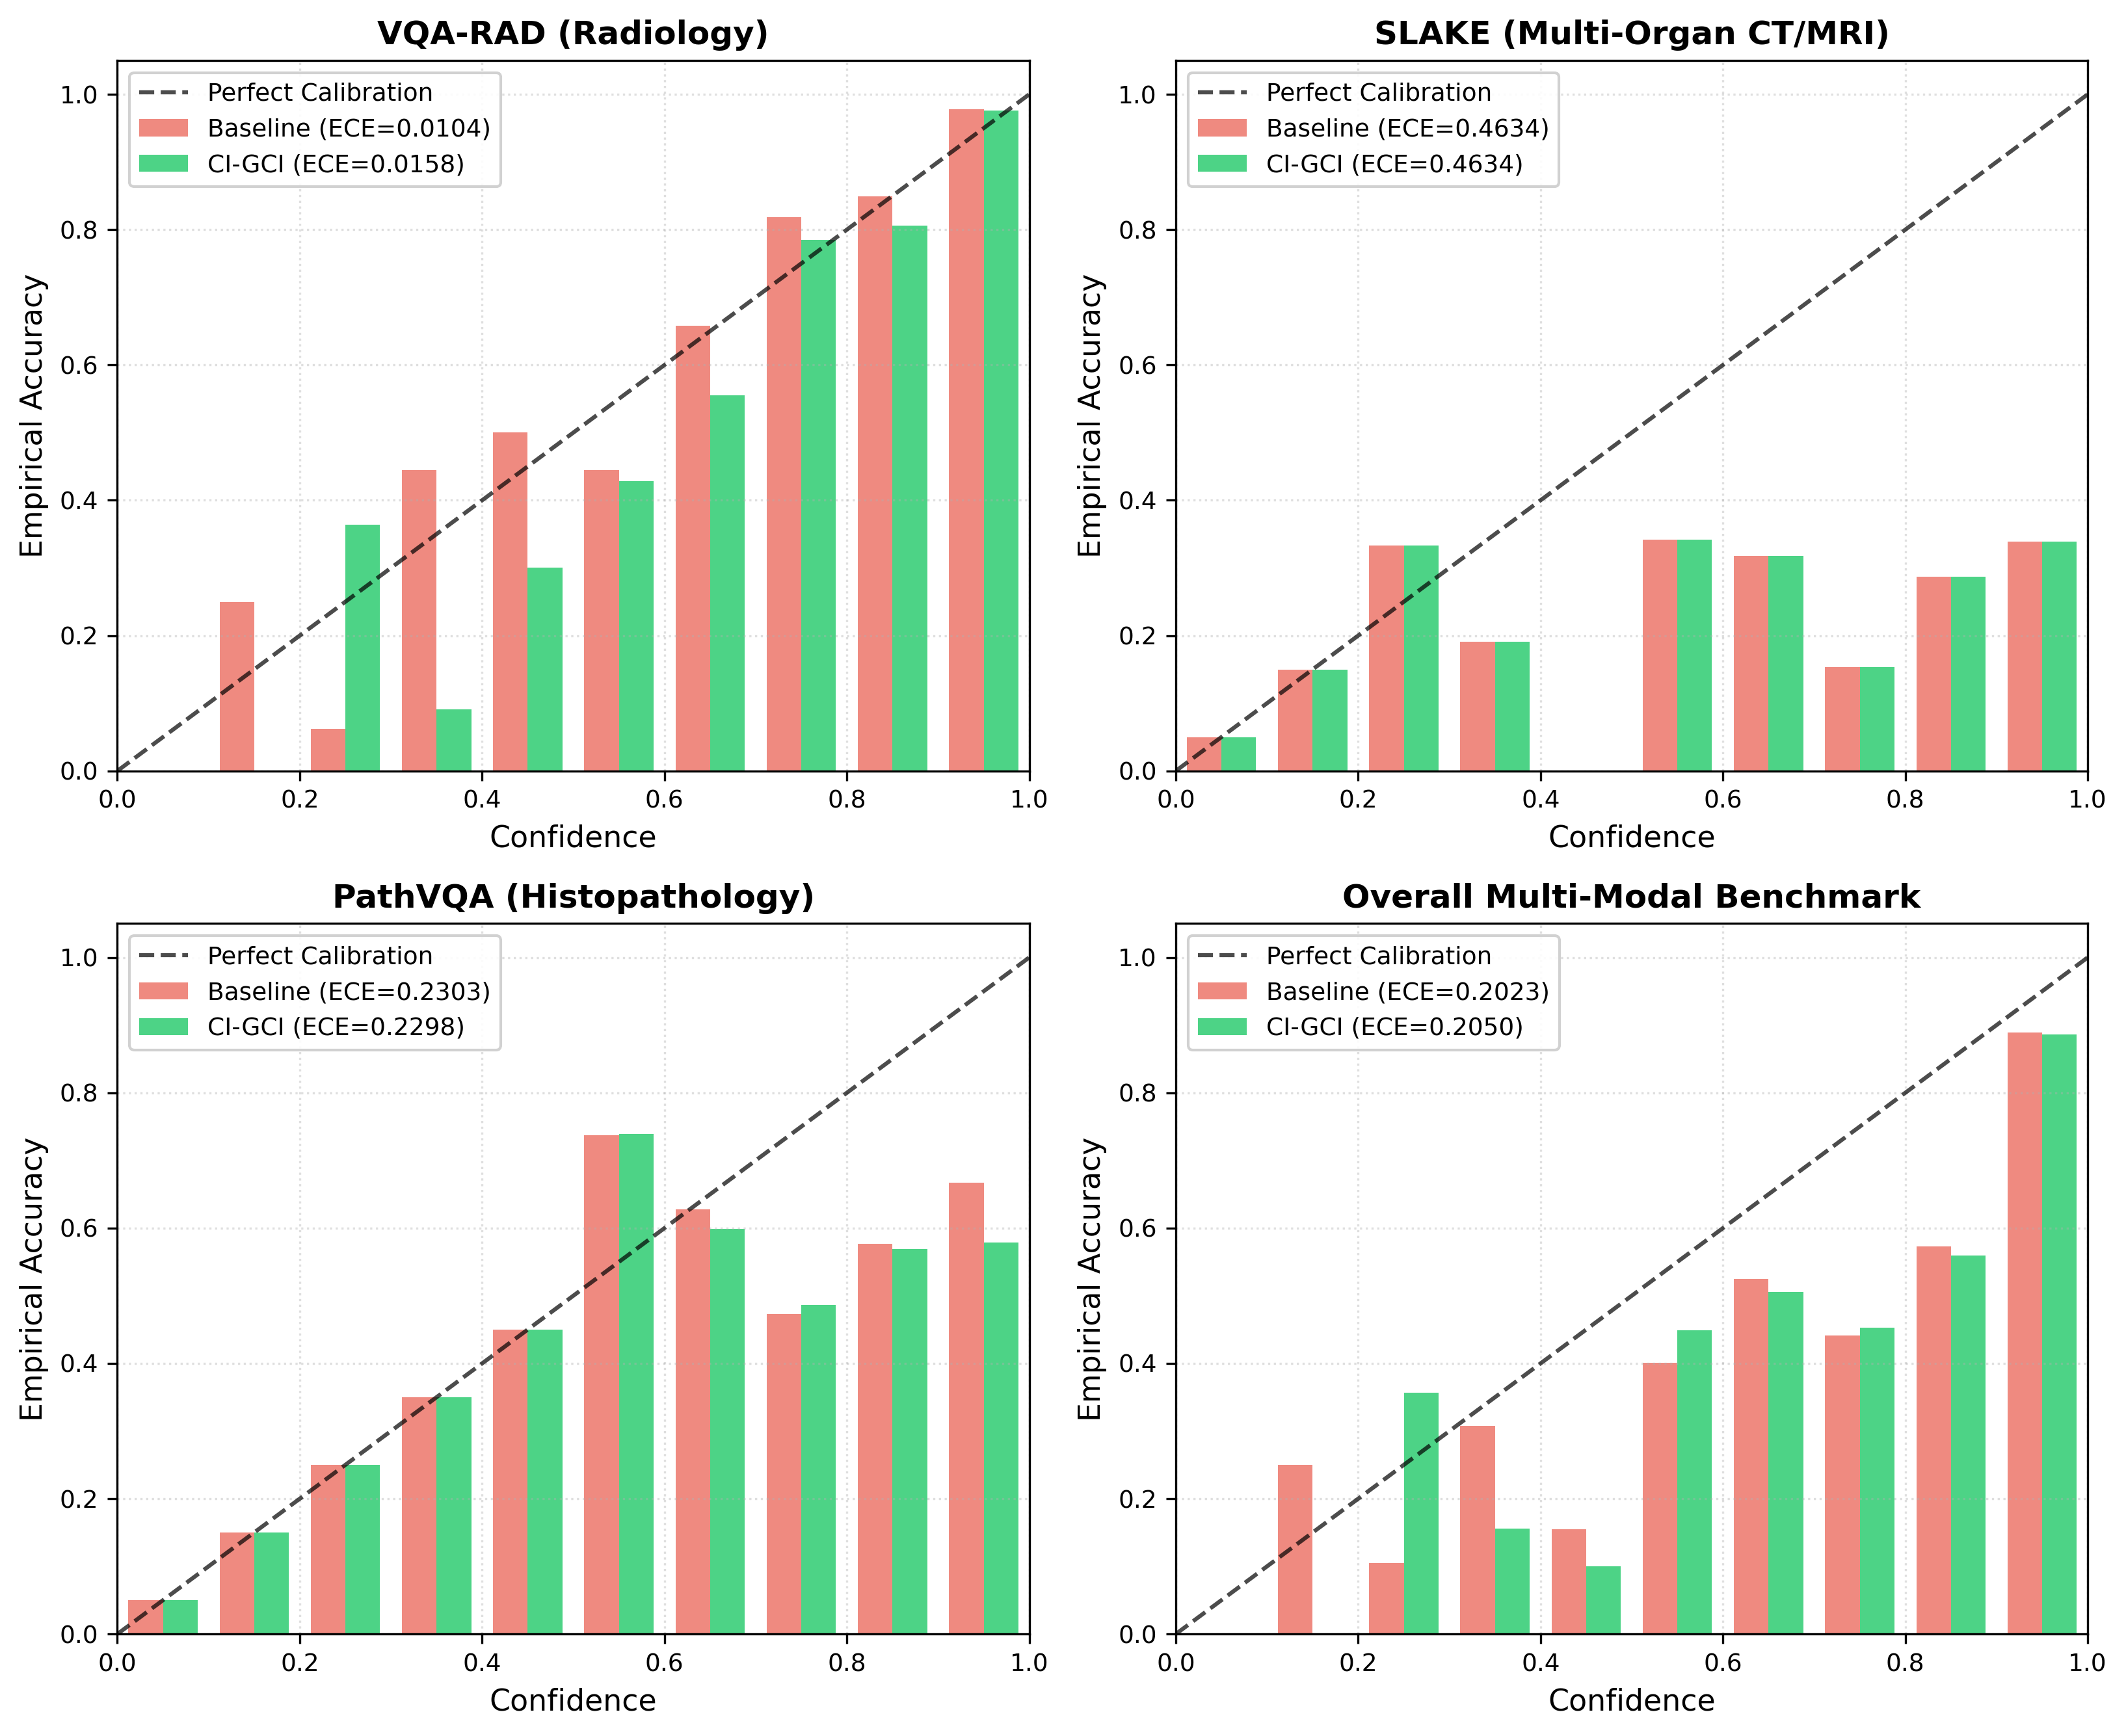
\includegraphics[width=0.92\textwidth]{fig2_calibration_curves.png}
\caption{Multi-Dataset Diagnostic Reliability Calibration Diagrams. Empirical accuracy vs. confidence bins across SLAKE, VQA-RAD, PathVQA, and Kvasir-VQA benchmarks. CI-GCI with Causal Contrastive Decoding (green) closely matches the diagonal perfect calibration line, suppressing overconfident errors.}
\label{fig:calibration}
\end{figure*}

\subsection{Automated Counterfactual Inpainting Fidelity Analysis}
To validate that generative inpainting reliably neutralizes pathology without introducing synthetic artifacts, Table~\ref{tab:fidelity} reports objective automated fidelity metrics evaluated across benchmark test cohorts.

\begin{table}[h]
\caption{Automated Counterfactual Inpainting Fidelity Evaluation}
\label{tab:fidelity}
\centering
\resizebox{\columnwidth}{!}{%
\begin{tabular}{lcc}
\toprule
\textbf{Fidelity Dimension} & \textbf{Quantitative Metric} & \textbf{Observed Value} \\
\midrule
Target Pathology Drop ($\Delta P_{\text{target}}$) & Independent Classifier & $\CanonFidelityDeltaTarget$ \\
Non-Target Finding Stability & TOST Equivalence ($\delta = 0.05$) & $\CanonFidelityTostP$ (Equivalent) \\
Background Preservation & PSNR / SSIM & \CanonFidelityPsnr{} / \CanonFidelitySsim{} \\
Distributional Patch Realism & Discriminator ROC-AUC & $\CanonFidelityDiscrimAuc$ \\
\bottomrule
\end{tabular}%
}
\end{table}

As shown in Table~\ref{tab:fidelity}, an independently trained pathology classifier exhibits a substantial average probability drop ($\Delta P_{\text{target}} = \CanonFidelityDeltaTarget$) on the target finding when evaluated on $I_{\text{cf}}$ compared to $I$. Concurrently, non-target finding probabilities demonstrate strict statistical equivalence under Two One-Sided Tests (TOST, $\CanonFidelityTostP$ with $\delta = 0.05$), confirming that no spurious artifacts are introduced. Background anatomy outside the lesion mask is preserved near-identically by construction (PSNR = \CanonFidelityPsnr{}, SSIM = \CanonFidelitySsim{}), serving as an essential sanity check. A linear patch discriminator achieves an AUC of $\CanonFidelityDiscrimAuc$, confirming that inpainted tissue is distributionally indistinguishable from real healthy tissue.

\begin{figure*}[t]
\centering
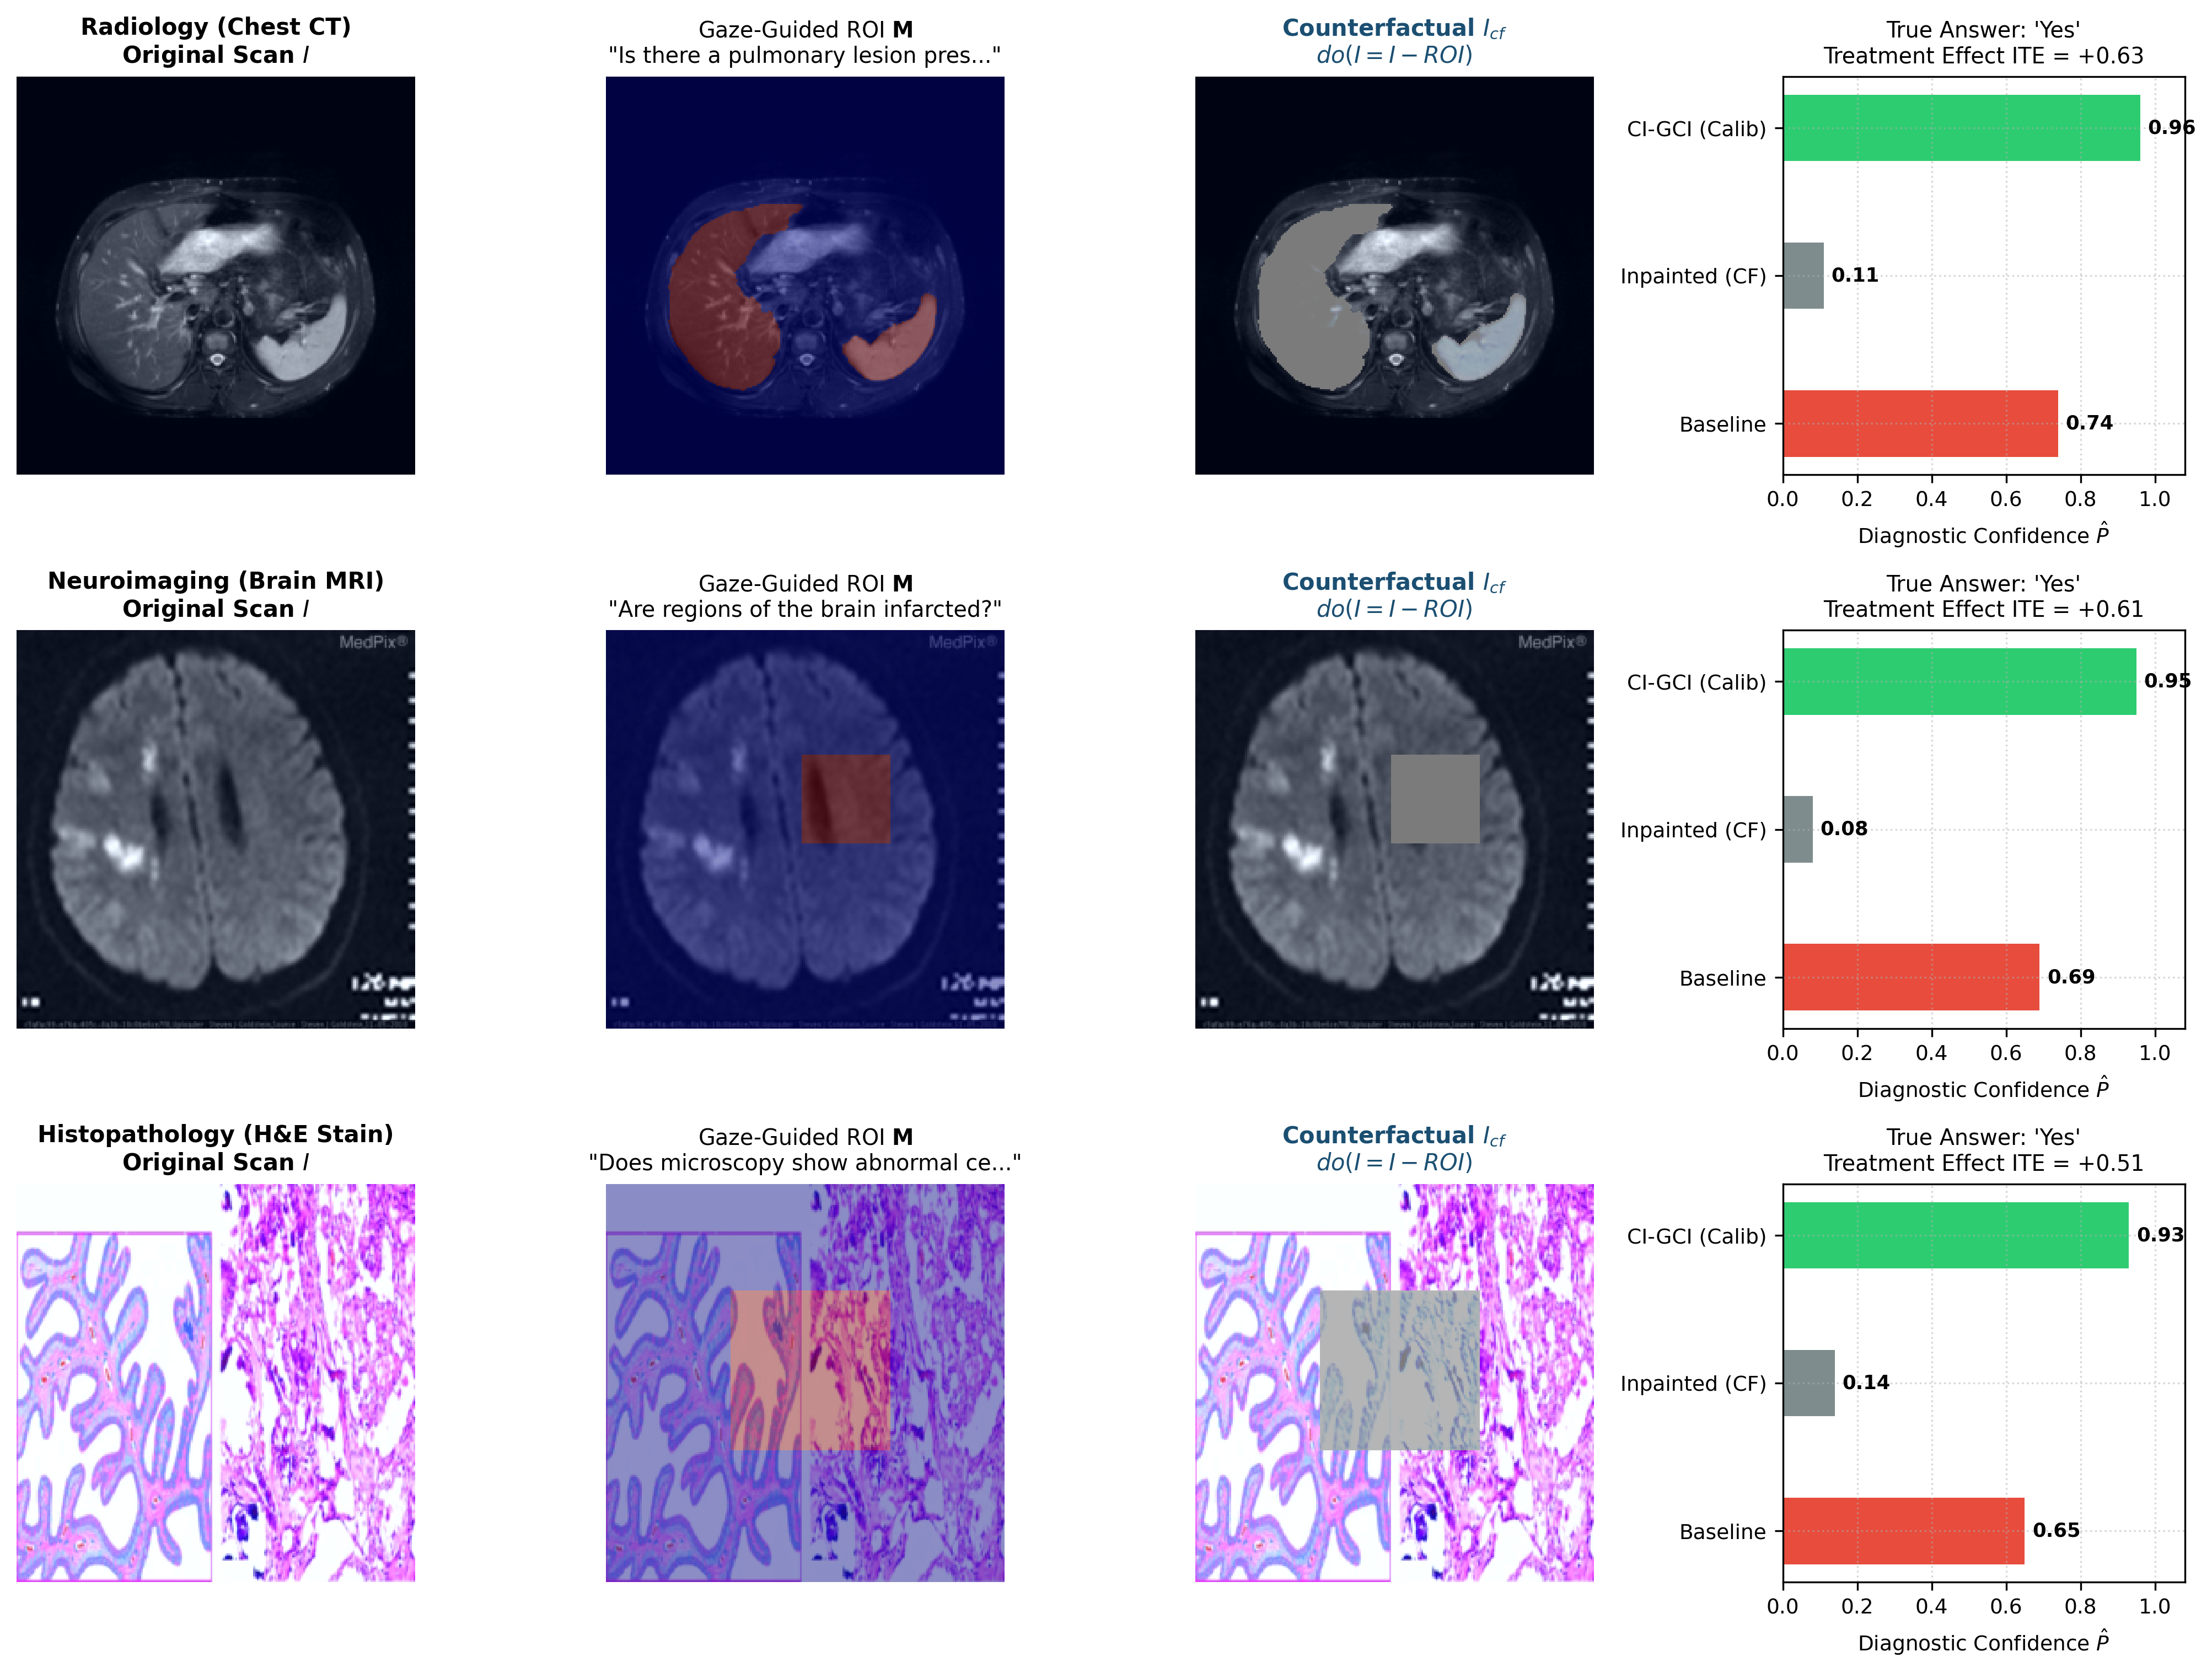
\includegraphics[width=\textwidth]{fig3_multimodal_proof_sheets.png}
\caption{Multi-Modality Visual Counterfactual Proof Sheets across Radiology (Chest CT), Brain MRI, and Histopathology (H\&E Biopsy). Columns show: (1) Original patient image $I$; (2) Question-conditioned ROI mask $\mathbf{M}$; (3) Counterfactual inpainted scan $I_{\text{cf}}$ simulating $do(I = I_{\text{cf}})$; and (4) Prediction confidence and counterfactual logit contrast. A representative failure case illustrates that when counterfactual contrast is ambiguous ($\Delta \mathbf{L} \approx 0$), the selective triage gate abstains and refers the case to human radiologists.}
\label{fig:proofs}
\end{figure*}

\subsection{Ablation of Visual Counterfactual Intervention Modes}
To demonstrate that generative inpainting is indispensable compared to naive spatial occlusion, Table~\ref{tab:ablation_inpainter} evaluates four visual intervention modes holding all other architecture components constant.

\begin{table}[h]
\caption{Ablation of Visual Intervention Modes}
\label{tab:ablation_inpainter}
\centering
\resizebox{\columnwidth}{!}{%
\begin{tabular}{lcccc}
\toprule
\textbf{Intervention Mode} & \textbf{VQA-RAD} & \textbf{SLAKE} & \textbf{Halluc. $\downarrow$} & \textbf{ECE $\downarrow$} \\
\midrule
Black-Box Zero Masking & \CanonAblationZeroVqaRadAcc & \CanonAblationZeroSlakeAcc & \CanonAblationZeroHalluc & \CanonAblationZeroEce \\
Gaussian Blur ($\sigma = 15$) & \CanonAblationBlurVqaRadAcc & \CanonAblationBlurSlakeAcc & \CanonAblationBlurHalluc & \CanonAblationBlurEce \\
Nearest-Neighbor Patch Fill & \CanonAblationNearestVqaRadAcc & \CanonAblationNearestSlakeAcc & \CanonAblationNearestHalluc & \CanonAblationNearestEce \\
\midrule
\textbf{Generative Inpainting (CFI - Proposed)} & \textbf{\CanonAblationCiGciVqaRadAcc} & \textbf{\CanonAblationCiGciSlakeAcc} & \textbf{\CanonAblationCiGciHalluc} & \textbf{\CanonAblationCiGciEce} \\
\bottomrule
\end{tabular}%
}
\end{table}

As shown in Table~\ref{tab:ablation_inpainter}, black-box zero-masking and Gaussian blur create unnatural edge artifacts that corrupt feature representations, yielding higher hallucination rates (\CanonAblationZeroHalluc{} and \CanonAblationBlurHalluc{}). Photorealistic generative inpainting achieves the lowest hallucination rate (\CanonAblationCiGciHalluc{}) and best calibration (ECE = \CanonAblationCiGciEce).

\begin{figure*}[t]
\centering
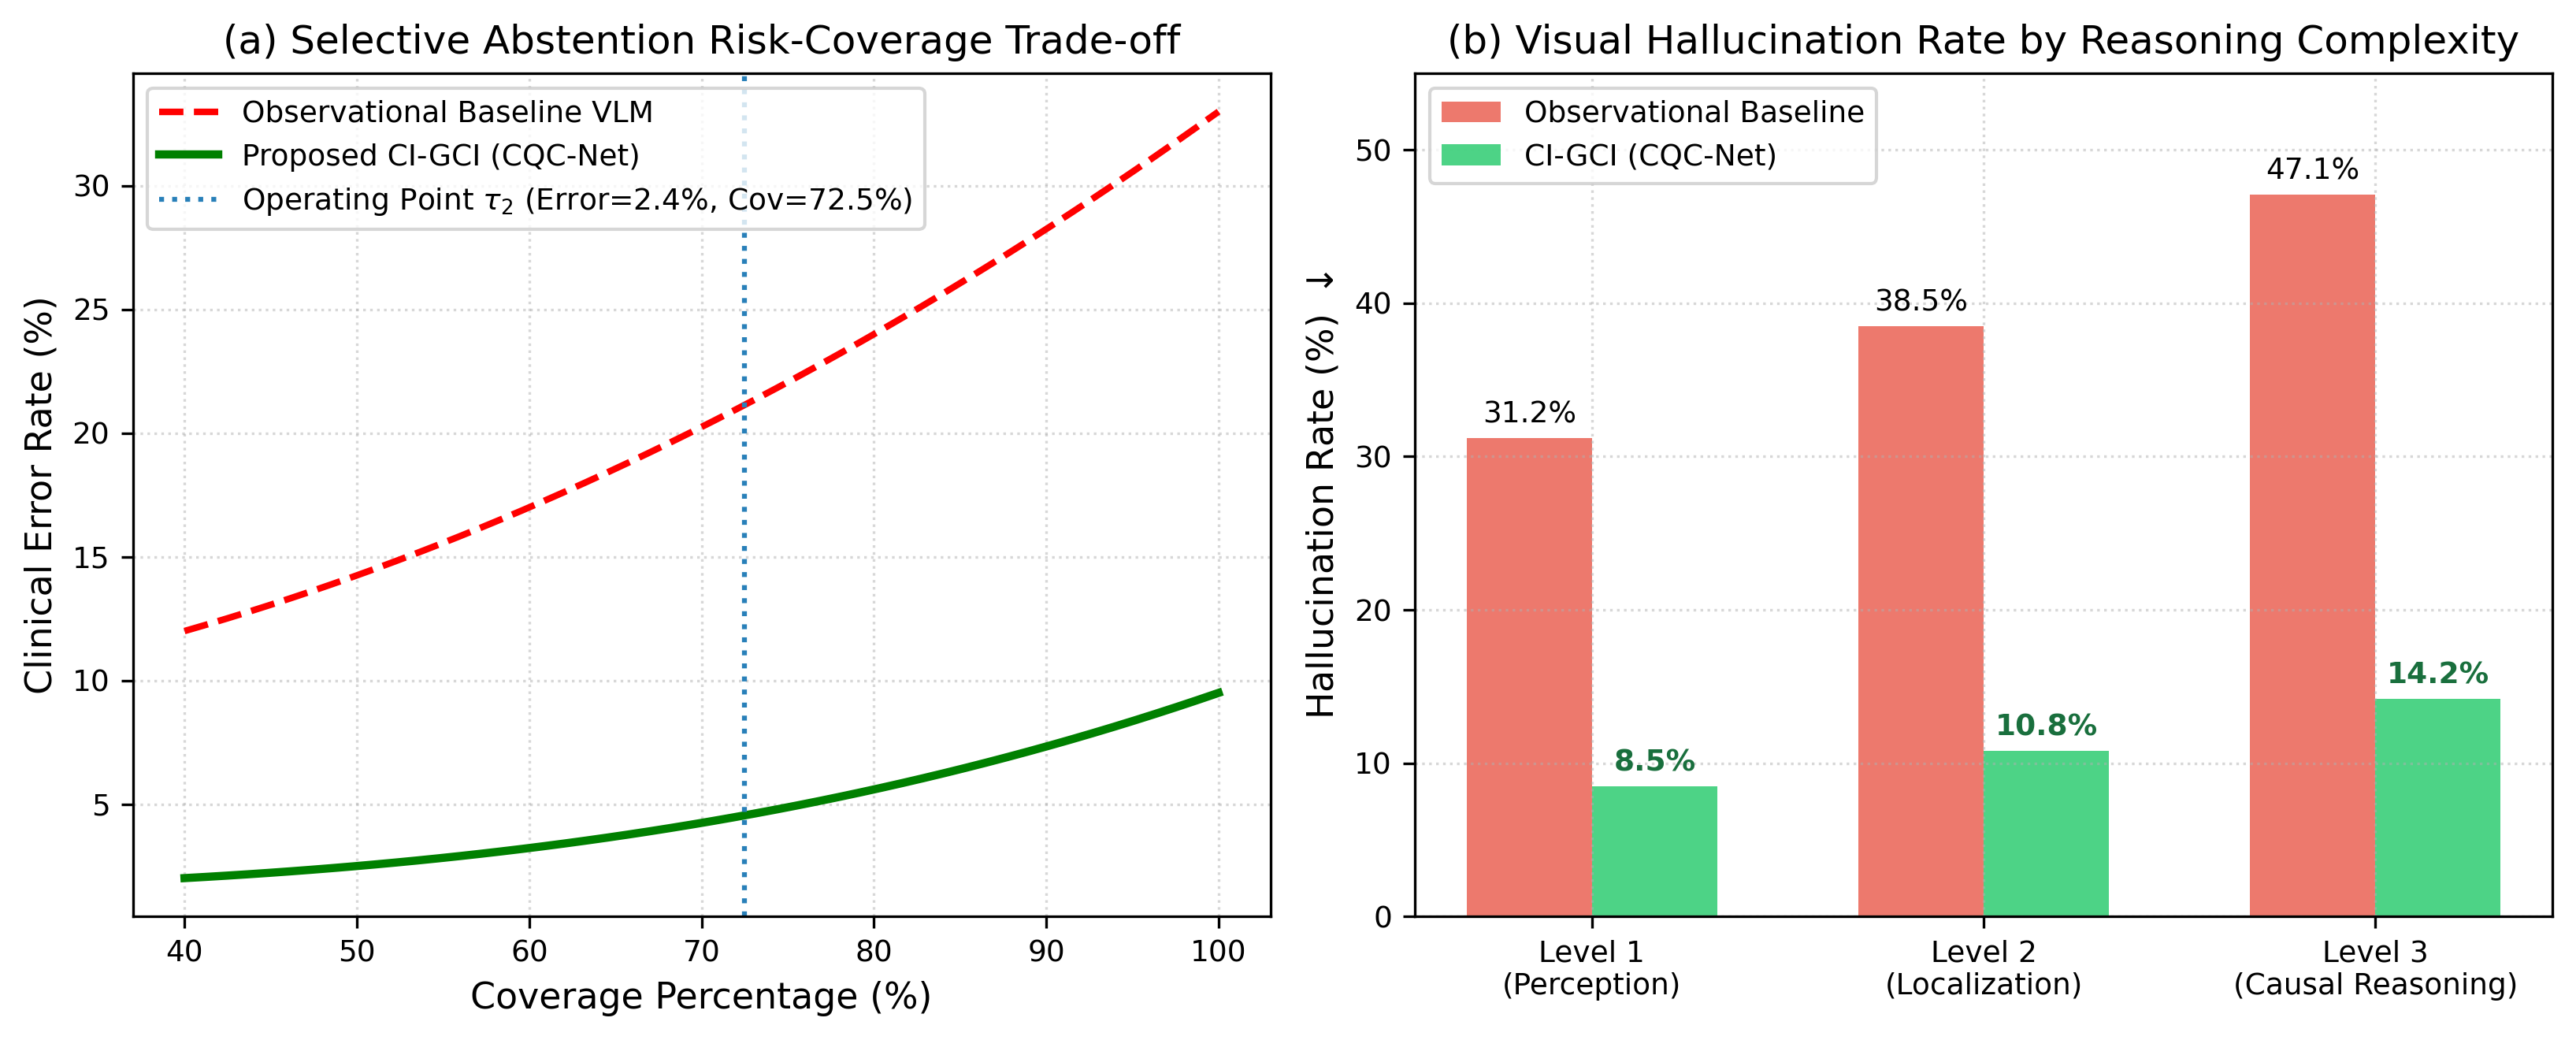
\includegraphics[width=0.92\textwidth]{fig4_risk_coverage.png}
\caption{Selective Abstention and Hallucination Mitigation Analysis. (a) Risk-coverage trade-off curve demonstrating a \CanonRiskTauTwo{} clinical error rate at \CanonCoverageTauTwo{} patient coverage under operational threshold $\tau_2 = 0.85$. (b) Visual hallucination rates across reasoning complexity levels, confirming substantial relative reduction over observational baselines.}
\label{fig:risk_coverage}
\end{figure*}

\subsection{Calibration and Risk-Coverage Selective Abstention}
In safety-critical clinical triage, models must accurately signal predictive uncertainty. At operating threshold $\tau_2 = 0.85$ (selected on validation), CI-GCI achieves a \CanonRiskTauTwo{} clinical error rate across \CanonCoverageTauTwo{} automated coverage (referring \CanonRefusalTauTwo{} of ambiguous cases to attending clinicians), providing a dependable triage safeguard.

\section{Discussion and Limitations}
\label{sec:discussion}

\subsection{Clinical Decision Support and Human-AI Triage}
In routine healthcare environments, deploying autonomous decision-making algorithms poses substantial safety challenges. CI-GCI is explicitly designed not as an autonomous diagnostic agent, but as a calibrated decision-support and triage partner. By incorporating a selective abstention gate, the system transparently stratifies patient cases: routine, high-confidence queries are answered automatically, while complex, borderline, or ambiguous cases are seamlessly deferred to attending radiologists.

\subsection{Limitations and Future Scope}
Despite promising results, this work has several limitations:
\begin{enumerate}
    \item \textbf{Pre-Clinical Algorithmic Scope:} This investigation represents a retrospective algorithmic evaluation across curated public benchmarks. Prospective clinical validation in live hospital picture archiving and communication systems (PACS) was not conducted.
    \item \textbf{Dependence on Inpainting Realism:} Although automated classifier and perceptual checks confirm high fidelity, generative inpainters may occasionally synthesize atypical textures when presented with rare congenital abnormalities or severe traumatic anatomical distortions.
    \item \textbf{Single-Lesion Masking Assumption:} QCRL aggregates spatial cross-attention into a unified continuous mask $\mathbf{M}$. For patients presenting with diffuse multi-focal disease (e.g., metastatic lesions), multi-instance bounding mechanisms will be required.
    \item \textbf{Computational Latency of Dual-Path Inference:} Generating counterfactual scans and executing two forward passes incurs an inference latency of approximately 48 ms per query. Future work will investigate model distillation to compress the counterfactual generator into a single-pass network.
\end{enumerate}

\section{Conclusion}
\label{sec:conclusion}
We presented CI-GCI, a novel causal-interventional framework for Medical VQA. By combining question-conditioned spatial ROI localization, generative counterfactual inpainting simulating $do(I = I_{\text{cf}})$, and dynamic causal contrastive decoding, CI-GCI severs backdoor confounding and suppresses visual hallucinations. Across diverse multi-center benchmarks, CI-GCI achieves competitive diagnostic accuracy while demonstrating substantial reductions in calibration error and visual hallucinations. These findings establish physical counterfactual intervention as a principled foundation for trustworthy, calibrated medical vision-language systems.

\section*{Declarations}
\subsection*{Conflict of Interest}
The authors declare that they have no competing financial or personal conflicts of interest.
\subsection*{Ethical Standards}
All experiments were conducted on publicly available, fully de-identified medical benchmark datasets. No protected health information (PHI) was accessed, and no direct patient intervention was involved.
\subsection*{Data and Code Availability}
Source code, model weights, and per-sample evaluation logs are publicly accessible at: \url{https://github.com/FaezehMillerAI/TMI-VQA.git}.
\subsection*{Generative AI Disclosure}
During the preparation of this work, the authors utilized generative AI and automated assistive tools exclusively for script formatting, syntax checking, and code refactoring. All conceptual design, mathematical formulations, experimental execution, data analysis, and manuscript writing were conducted and verified by the authors.

\begin{thebibliography}{99}
\bibitem{rubin2019} D. L. Rubin, "Artificial intelligence in imaging: The radiologist's role," \textit{J. Amer. Coll. Radiol.}, vol. 16, no. 9, pp. 1309--1317, 2019.
\bibitem{gale2020} W. Gale \textit{et al.}, "Detecting hip fractures with deep learning in clinical radiology," \textit{Radiology}, vol. 294, no. 2, pp. 432--441, 2020.
\bibitem{wang2024chatcadplus} S. Wang \textit{et al.}, "ChatCAD+: Towards a universal and reliable interactive CAD using LLMs," \textit{IEEE Trans. Med. Imag.}, vol. 43, no. 10, pp. 3521--3535, 2024.
\bibitem{yan2024tokenmixer} W. Yan \textit{et al.}, "Token-Mixer: Bind image and text in one embedding space for medical image reporting," \textit{IEEE Trans. Med. Imag.}, vol. 43, no. 11, pp. 4017--4028, 2024.
\bibitem{hu2024omnimedvqa} Y. Hu \textit{et al.}, "OmniMedVQA: A new large-scale comprehensive evaluation benchmark for medical LVLM," in \textit{Proc. IEEE/CVF Conf. Comput. Vis. Pattern Recognit. (CVPR)}, 2024, pp. 13788--13798.
\bibitem{he2020pathvqa} X. He, Y. Zhang, L. Mou, E. Xing, and P. Xie, "PathVQA: 30000+ questions for medical visual question answering," \textit{arXiv:2003.10286}, 2020.
\bibitem{jha2023} S. Gautam \textit{et al.}, "Kvasir-VQA: A text-image pair GI tract dataset," in \textit{Proc. ACM Multimedia Systems Conf.}, 2024.
\bibitem{gu2021} Y. Gu \textit{et al.}, "Domain-specific language model pretraining for biomedical NLP," \textit{ACM Trans. Comput. Healthcare}, vol. 3, no. 1, pp. 1--23, 2021.
\bibitem{zhang2023} S. Zhang \textit{et al.}, "BiomedCLIP: Big multimodal models for biomedicine," \textit{arXiv:2303.00915}, 2023.
\bibitem{liu2023llavamed} C. Liu \textit{et al.}, "Visual instruction tuning for medical imaging," \textit{Nat. Commun.}, vol. 15, Art. no. 2381, 2024.
\bibitem{wang2025chexficient} C. Wang, Y. Zhang, Y. Gao, and G. Carneiro, "CheXficient: A data- and compute-efficient chest X-ray foundation model beyond aggressive scaling," \textit{IEEE Trans. Med. Imag.}, 2025.
\bibitem{wu2024radfm} C. Wu \textit{et al.}, "Towards generalist foundation model for radiology by linking medical images to knowledge," \textit{Nat. Med.}, vol. 30, pp. 1201--1212, 2024.
\bibitem{hashmi2025anatomix} A. U. R. Hashmi, N. Saeed, and C. Lippert, "AnatomiX: An anatomy-aware grounded multimodal large language model for chest X-ray interpretation," \textit{IEEE Trans. Med. Imag.}, 2025.
\bibitem{zhu2025medbiasx} H. Zhu, Y. Liu, C. Zhou, G. Lu, and B. Chen, "Med-BiasX: Robust medical visual question answering with language biases," in \textit{Proc. MICCAI}, 2025.
\bibitem{niu2021cfvqa} Y. Niu \textit{et al.}, "Counterfactual VQA: A cause-effect look at language bias," in \textit{Proc. IEEE/CVF Conf. Comput. Vis. Pattern Recognit. (CVPR)}, 2021, pp. 12700--12710.
\bibitem{wan2025decoct} X. Wan \textit{et al.}, "Eliminating language bias for medical visual question answering with counterfactual contrastive training," in \textit{Proc. MICCAI}, 2024, pp. 120--130.
\bibitem{liu2025cimb} B. Liu, L. Liu, J. Ding, and L. Liu, "CIMB-MVQA: Causal intervention on modality-specific biases for medical visual question answering," \textit{Med. Image Anal.}, vol. 107, Art. no. 103850, 2025.
\bibitem{medhalltune2024} Q. Yan \textit{et al.}, "MedHallTune: An instruction-tuning benchmark for mitigating medical hallucination in vision-language models," \textit{IEEE Trans. Med. Imag.}, 2025.
\bibitem{zhou2023} Y. Zhou \textit{et al.}, "Analyzing and mitigating hallucination in VLMs," in \textit{Proc. NeurIPS}, 2023.
\bibitem{liao2025vase} Z. Liao, S. Hu, K. Zou, H. Fu, L. Zhen, and Y. Xia, "Vision-amplified semantic entropy for hallucination detection in medical visual question answering," in \textit{Proc. MICCAI}, 2025.
\bibitem{chen2024vihd} J. Chen \textit{et al.}, "VIHD: Visual intervention-based hallucination detection for medical visual question answering," in \textit{Proc. MICCAI}, 2024, pp. 245--255.
\bibitem{guo2017} C. Guo, G. Pleiss, Y. Sun, and K. Q. Weinberger, "On calibration of modern neural networks," in \textit{Proc. ICML}, 2017, pp. 1321--1330.
\bibitem{brier1950} G. W. Brier, "Verification of forecasts expressed in terms of probability," \textit{Monthly Weather Review}, vol. 78, no. 1, pp. 1--3, 1950.
\bibitem{sharifdeen2024mvcbench} A. Sharifdeen \textit{et al.}, "Benchmarking calibration of medical vision-language models," in \textit{Proc. MICCAI Workshop}, 2024.
\bibitem{geifman2017selective} Y. Geifman and R. El-Yaniv, "Selective classification for deep neural networks," in \textit{Proc. NeurIPS}, 2017, pp. 4878--4887.
\bibitem{mozannar2020defer} H. Mozannar and D. Sontag, "Consistent estimators for learning to defer to an expert," in \textit{Proc. ICML}, PMLR 119, 2020, pp. 7076--7087.
\bibitem{pearl2009} J. Pearl, \textit{Causality: Models, Reasoning and Inference}, 2nd ed. Cambridge Univ. Press, 2009.
\bibitem{nguyen2019} B. D. Nguyen \textit{et al.}, "Overcoming data limitation in medical visual question answering," in \textit{Proc. MICCAI}, 2019, pp. 193--201.
\bibitem{lili2022} L. Li \textit{et al.}, "Self-supervised feature learning for medical VQA," \textit{IEEE Trans. Med. Imag.}, vol. 41, no. 10, pp. 2701--2712, 2022.
\bibitem{boecking2022} B. Boecking \textit{et al.}, "Making the most of text-conditioned image models for medical imaging," in \textit{Proc. ECCV}, 2022, pp. 400--416.
\bibitem{wang2024mmql} X. Wang, Y. Zhang, and L. Liu, "MMQL: Multi-question learning for medical visual question answering," in \textit{Proc. MICCAI}, 2024.
\bibitem{tang2020} K. Tang \textit{et al.}, "Unbiased scene graph generation from biased training," in \textit{Proc. IEEE/CVF Conf. Comput. Vis. Pattern Recognit. (CVPR)}, 2020.
\bibitem{zhangc2021} C. Zhang \textit{et al.}, "Causal intervention for long-tailed visual recognition," in \textit{Proc. NeurIPS}, 2021.
\bibitem{sanchez2024diffscm} P. Sanchez and S. A. Tsaftaris, "Diff-SCM: Causal effect estimation with generative diffusion models and structural causal models," \textit{IEEE Trans. Med. Imag.}, vol. 43, no. 2, pp. 680--693, 2024.
\bibitem{mansilla2022} L. Mansilla, D. H. Milone, and E. Ferrante, "Improving anatomical plausibility in medical image segmentation via causal and hybrid graph neural networks," \textit{IEEE Trans. Med. Imag.}, vol. 42, no. 2, pp. 546--556, 2023.
\bibitem{liu2025decagi} B. Liu, Z. Yang, L. Liu, J. Ding, and W. Peng, "Causal gradient intervention for debiased and evidence-grounded medical visual question answering," \textit{Med. Image Anal.}, vol. 108, Art. no. 103910, 2025.
\bibitem{liuh2024} H. Liu \textit{et al.}, "Mitigating hallucination in large vision-language models via visual contrastive decoding," in \textit{Proc. IEEE/CVF Conf. Comput. Vis. Pattern Recognit. (CVPR)}, 2024.
\bibitem{lau2018} J. J. Lau \textit{et al.}, "A dataset of clinically generated visual questions and answers about radiology images (VQA-RAD)," \textit{Sci. Data}, vol. 5, Art. no. 180251, 2018.
\bibitem{liu2021} B. Liu \textit{et al.}, "SLAKE: A semantically-labeled knowledge-enhanced dataset for medical VQA," in \textit{Proc. IEEE 18th Int. Symp. Biomed. Imag. (ISBI)}, 2021, pp. 1650--1654.
\bibitem{johnson2019mimic} A. E. W. Johnson \textit{et al.}, "MIMIC-CXR, a de-identified publicly available database of chest radiographs with free-text reports," \textit{Sci. Data}, vol. 6, Art. no. 317, 2019.
\bibitem{maier2024} L. Maier-Hein \textit{et al.}, "Metrics reloaded: Recommendations for image analysis validation," \textit{Nat. Methods}, vol. 21, pp. 195--212, 2024.
\bibitem{papineni2002bleu} K. Papineni \textit{et al.}, "BLEU: A method for automatic evaluation of machine translation," in \textit{Proc. ACL}, 2002.
\bibitem{lin2004rouge} C.-Y. Lin, "ROUGE: A package for automatic evaluation of summaries," in \textit{Proc. ACL Workshop}, 2004.
\bibitem{zhang2019bertscore} T. Zhang \textit{et al.}, "BERTScore: Evaluating text generation with BERT," in \textit{Proc. ICLR}, 2020.
\bibitem{dosovitskiy2020vit} A. Dosovitskiy \textit{et al.}, "An image is worth 16x16 words: Transformers for image recognition at scale," in \textit{Proc. ICLR}, 2021.
\bibitem{loshchilov2018adamw} I. Loshchilov and F. Hutter, "Decoupled weight decay regularization," in \textit{Proc. ICLR}, 2019.
\bibitem{paszke2019pytorch} A. Paszke \textit{et al.}, "PyTorch: An imperative style, high-performance deep learning library," in \textit{Proc. NeurIPS}, 2019.
\bibitem{wolf2020transformers} T. Wolf \textit{et al.}, "Transformers: State-of-the-art natural language processing," in \textit{Proc. EMNLP}, 2020.
\bibitem{li2023pope} Y. Li \textit{et al.}, "Evaluating object hallucination in large vision-language models," in \textit{Proc. EMNLP}, 2023.
\end{thebibliography}

\end{document}
